\documentclass[twocolumn]{article}

\usepackage{graphicx}

\title{Analise dos dados do experimento XXX}
\author{Eu et galera}

\begin{document}

\maketitle


\section{Abstract}

Meh.

\section{Introduction}

Bla.

\section{Methods}

See the IPython notebook file.

\section{Results}

My results:


\begin{figure}[!hb]
    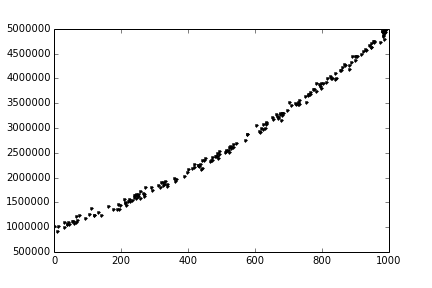
\includegraphics[scale=0.5]{notebook/dados.png}
    \caption{The data.}
\end{figure}

\begin{figure}[!hb]
    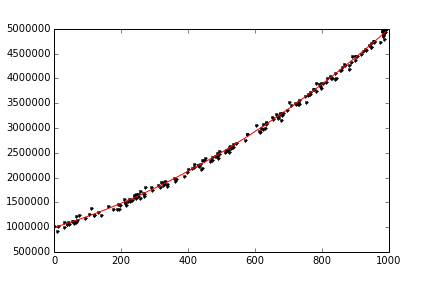
\includegraphics[scale=0.5]{notebook/ajuste.png}
    \caption{The adjustment.}
\end{figure}

\end{document}
